\section{Análisis exploratorio}

\paragraph{Tendencia}
Como podemos ver en la figura \ref{ea_plot} los gráficos de dispersión de los datos frente a las coordenadas podemos asumir que no hay tendencia, ya que parece que no hay un patrón definido con los puntos.  

\begin{figure}
    \centering
    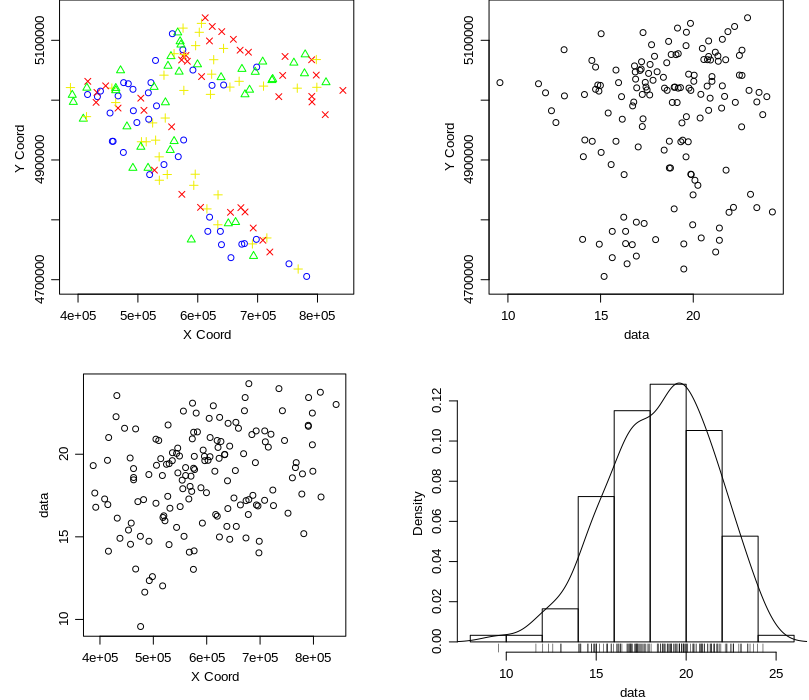
\includegraphics[scale=0.4]{geoestadistica/proyectos/proyecto_geoestadistica_croacia/images/ae_plot.png}
    \caption{Gráficos de dispersión e histograma de temperatura media para 14/04/2008 en Croacia }
    \label{ea_plot}
\end{figure}


